%%%%%%%%%%%%%%%%%%%%%%%%%%%%%%%%%%%%%%%%%%%%%%%%%%%%%
%
%  Template
%  Beamer Presentation by Chris Bourke
%
%%%%%%%%%%%%%%%%%%%%%%%%%%%%%%%%%%%%%%%%%%%%%%%%%%%%%%%%%%%%%%%%%%%%%%%

\documentclass[]{beamer}
%\documentclass[handout]{beamer}

\geometry{papersize={16cm,9cm}}

% For handout version:
%\usetheme[hideothersubsections,slidenumbers]{UNLTheme}
\usetheme[hideothersubsections]{UNLTheme}
\usepackage{amssymb}
\input{StandardCommands}
\usepackage[linesnumbered,ruled,vlined]{algorithm2e}
\SetKwComment{Comment}{//}{}
\DontPrintSemicolon
\SetKwSty{textsc} %
%\SetAlFnt{\scriptsize} %
\SetKwInOut{Input}{Input} %
\SetKwInOut{Output}{Output} %
%\setalcapskip{1em} % changed to
\SetAlCapSkip{1em}
\setlength{\algomargin}{2em} %
%\Setvlineskip{0em} % changed to:
\SetVlineSkip{0em}

\usepackage{tikz}

\definecolor{steelblue}{rgb}{0.2745,0.5098,0.7059}
\definecolor{limegreen}{RGB}{50,205,50}
\hypersetup{
    colorlinks = true,
    urlcolor = {steelblue},
    linkbordercolor = {white}
}

\definecolor{mintedBackground}{rgb}{0.95,0.95,0.95}
\definecolor{mintedInlineBackground}{rgb}{.90,.90,1}

%\usepackage{newfloat}
\usepackage{minted}
\setminted{mathescape,
               linenos,
               autogobble,
               frame=none,
               fontsize=\small,
               framesep=2mm,
               framerule=0.4pt,
               %label=foo,
               xleftmargin=2em,
               xrightmargin=0em,
               startinline=true,  %PHP only, allow it to omit the PHP Tags *** with this option, variables using dollar sign in comments are treated as latex math
               numbersep=10pt, %gap between line numbers and start of line
               style=default, %syntax highlighting style, default is "default"
               			    %gallery: http://help.farbox.com/pygments.html
			    	    %list available: pygmentize -L styles
               bgcolor=mintedBackground} %prevents breaking across pages
               
\setmintedinline{bgcolor={mintedInlineBackground}}
\setminted[text]{bgcolor={},linenos=false,autogobble,xleftmargin=1em}

\usetikzlibrary{decorations.pathreplacing,arrows}
\usetikzlibrary{patterns}
\usetikzlibrary{arrows,arrows.meta,backgrounds,calc,trees,decorations,decorations.pathmorphing}

\title[~]{Computer Science I}
\subtitle{Searching \& Sorting}
\author[~]{Dr.\ Chris Bourke\\ \email{cbourke@cse.unl.edu}} %
\date{~}

\begin{document}

\begin{frame}
  \titlepage
\end{frame}

\setbeamertemplate{section in toc}{\inserttocsectionnumber.~\inserttocsection}
\setbeamercolor{section in toc}{fg=black}
%\setbeamertemplate{subsection in toc}{~} %\inserttocsubsection\\}

\begin{frame}
  \frametitle{Outline}
%{\footnotesize
%\begin{NoHyper}
%  \tableofcontents[hideallsubsections]
%\end{NoHyper}
%}

\setbeamercolor{enumerate item}{bg=white,fg=black}
\setbeamercolor{item}{bg=white,fg=black}
\setbeamercolor{item projected}{bg=white,fg=black}
\setbeamercolor{enumerate subitem}{fg=red!80!black}
\setbeamertemplate{enumerate items}[default]
\begin{enumerate}
  \item Introduction \& Linear Search
   %intro
   %linear search, can we do better?
  \item Binary Search 
   %binary search
   %analysis/comparison of linear vs binary search
  \item Sorting: Selection Sort
  \item Sorting: Quick Sort
    %quick sort
    %other sorts
  \item Sorting in Practice
    %comaprator functions
  \item Function Pointers
  \item Searching \& Sorting in C
   %generic linear search    
   %qsort
   %bsearch
\end{enumerate}

\end{frame}

\section{Introduction}

\begin{frame}
    \frametitle{}
    \framesubtitle{}
    
    \begin{center}
    {\Huge Part I: Introduction \& Linear Search}\\
    {\Large ~}
    \end{center}

\end{frame}

\begin{frame}[fragile]
  \frametitle{Introduction}
  \framesubtitle{}

\begin{itemize}[<+->]
  \item Processing data is a fundamental operation in Computer Science
  \item Two fundamental operations in processing data are \emph{searching} 
   and \emph{sorting}
  \item Form the basis or preprocessing step of many algorithms
  \item Large variety of algorithms have been developed
\end{itemize}

\end{frame}

\begin{frame}[fragile]
  \frametitle{Searching}
  \framesubtitle{}

\begin{itemize}[<+->]
  \item Given a \emph{collection} of \emph{elements} 
  $A = \{a_1, a_2, \ldots, a_n\}$ and a \emph{key} $k$, find an element 
  that ``matches'' $k$
  \item Collection: haystack, key: needle
\end{itemize}

\end{frame}

\begin{frame}[fragile]
  \frametitle{Searching}
  \framesubtitle{}

Very general problems statement:
\begin{itemize}[<+->]
  \item Collection: arrays, sets, lists, etc.
  \item Elements: integers, strings, structures, etc.
  \item ``matches'': could be any criteria!
  \item Variations:
  \begin{itemize}
    \item Find the first/last such element
    \item Find all such elements
    \item Find extremal elements
  \end{itemize}
  \item What do you do for unsuccessful searches?
\end{itemize}

\end{frame}

\begin{frame}[fragile]
  \frametitle{Linear Search}
  \framesubtitle{}

Potential Solution: Linear Search
\begin{itemize}[<+->]
  \item Basic idea: iterate through each element
  \item For each element, apply the ``matching'' criteria
  \item Stop at the first match
  \item If no such element, return a ``flag'' value
\end{itemize}

\end{frame}

\begin{frame}[fragile]
  \frametitle{Linear Search}
  \framesubtitle{}

A potential C solution:
\begin{itemize}[<+->]
  \item Take an array of integers 
  \item An integer key $k$
  \item Find the first element equal to $k$
  \item Return its index
  \item Unsuccessful search: $-1$ as a flag value
\end{itemize}

\end{frame}

\begin{frame}[fragile]
  \frametitle{Linear Search}
  \framesubtitle{}

\begin{minted}[fontsize=\scriptsize]{c}
/**
 * This function takes an array of integers
 * and searches it for the given key, returning
 * the index at which it finds it, or -1 if no
 * such element exists.
 */
int linearSearch(const int *arr, int n, int key) {

  for(int i=0; i<n; i++) {
    if(arr[i] == key) {
      //you found your needle...
      return i;
    }
  }
  //the needle was not found
  return -1;
}
\end{minted}

\end{frame}

\begin{frame}[fragile]
  \frametitle{Linear Search: Observations}
  \framesubtitle{}

Solution works
\begin{itemize}[<+->]
  \item Solution works but is less than ideal
  \item It only applies to arrays of integers
  \item Search arrays of \mintinline{c}{double} or strings or
  \mintinline{c}{Student} structures, etc.: copy-pasta
  \item Different search criteria (search \mintinline{c}{Student} by NUID or name): yet another implementation
  \item Ultimate goal: one single ``generic'' searching (and sorting) solution that will work with arrays of any type of data
  \item Can we do better? %before we tackle that problem
\end{itemize}

\end{frame}

\section{Binary Search}

\begin{frame}
    \frametitle{}
    \framesubtitle{}
    
    \begin{center}
    {\Huge Part II: Binary Search \& Comparison}\\
    {\Large ~}
    \end{center}

\end{frame}

\begin{frame}[fragile]
  \frametitle{Binary Search: Basic Idea}
  \framesubtitle{}

\begin{itemize}[<+->]
  \item Can we do better than linear search?
  \item Suppose that the array is \emph{sorted}: how might we exploit that structure?
  \item Searching for an element $k$
  \item Examine the middle element, $m$:
  \begin{itemize}
    \item If $m = k$: success!
    \item If $k < m$: $k$ must lie in the left-half of the array
    \item If $m < k$: $k$ must lie in the right-half of the array
  \end{itemize}
\end{itemize}

\end{frame}

\begin{frame}[fragile]
  \frametitle{Illustration}
  \framesubtitle{}

\begin{center}
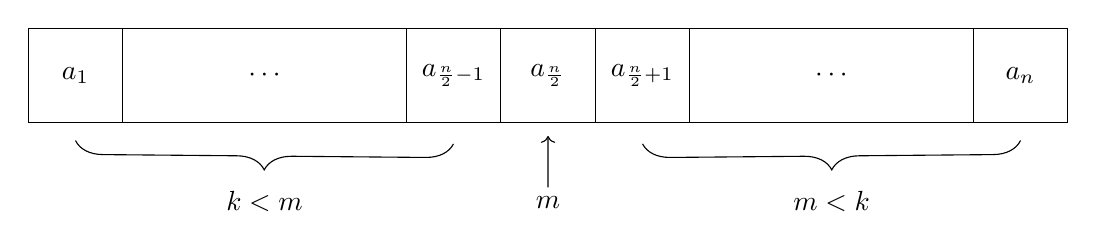
\begin{tikzpicture}[scale=1.2]

\draw (0,0) rectangle (1,1);
\node (a) at (0.5, 0.5) {$a_1$};

\draw (1,0) rectangle (4,1);
\node at (2.5, 0.5) {$\cdots$};

\draw (4,0) rectangle (5,1);
\node (b) at (4.5, 0.5) {$a_{\frac{n}{2}-1}$};

\draw (5,0) rectangle (6,1);
\node (am) at (5.5, 0.5) {$a_{\frac{n}{2}}$};

\draw (6,0) rectangle (7,1);
\node (c) at (6.5, 0.5) {$a_{\frac{n}{2}+1}$};

\draw (7,0) rectangle (10,1);
\node at (8.5, 0.5) {$\cdots$};

\draw (10,0) rectangle (11,1);
\node (d) at (10.5, 0.5) {$a_{n}$};


\node (m) at (5.5, -0.85) {$m$};
\draw[->,shorten >=0.5cm] (m) -- (am);


  \draw [decorate,decoration={brace,mirror,amplitude=10pt},xshift=-4pt,yshift=0pt] ([xshift=0cm,yshift=-.5cm]a.south) -- ([xshift=0cm,yshift=-0.5cm]b.south) node [black,midway,yshift=-0.75cm] {$k < m$};

  \draw [decorate,decoration={brace,mirror,amplitude=10pt},xshift=-4pt,yshift=0pt] ([xshift=0cm,yshift=-.5cm]c.south) -- ([xshift=0cm,yshift=-0.5cm]d.south) node [black,midway,yshift=-0.75cm] {$m < k$};


\end{tikzpicture}
\end{center}

\end{frame}

\begin{frame}[fragile]
  \frametitle{Example}
  \framesubtitle{}%1
  
Search for $k = 42$:
$$l = 0, \quad r = 10, \quad m = 5$$

\begin{center}
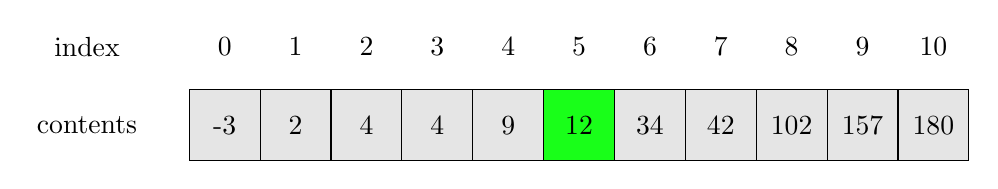
\begin{tikzpicture}
% size of each node
\def\sz{9mm}
% node style definition
\tikzstyle{block} = [
	draw, fill=black!10, rectangle,
	minimum height=\sz, minimum width=\sz ];
\tikzstyle{plain} = [draw=none,fill=none];
% array element definition
\def\arr{0, 2, 4, 4, 9, 12, 34, 42, 102};
%\def\x{0}; % x pos of arr
%\def\y{0}; % y pos of arr
%\newcounter{ind};
%\setcounter{ind}{0};
\node[plain] at (-1.75, 1) { index };
\node[plain] at (-1.75, 0) { contents };

\node[block] at (0,0) { -3 };
\node[plain] at (0,1.0) { 0 };

\node[block] at (1*\sz,0) { 2 };
\node[plain] at (1*\sz,1.0) { 1 };

\node[block] at (2*\sz,0) { 4 };
\node[plain] at (2*\sz,1.0) { 2 };

\node[block] at (3*\sz,0) { 4 };
\node[plain] at (3*\sz,1.0) { 3 };

\node[block] at (4*\sz,0) { 9 };
\node[plain] at (4*\sz,1.0) { 4 };

\node[block] at (5*\sz,0) { 12 };
\onslide<2->{\node[block,fill=white!10!green] at (5*\sz,0) { 12 };}
\node[plain] at (5*\sz,1.0) { 5 };

\node[block] at (6*\sz,0) { 34 };
\node[plain] at (6*\sz,1.0) { 6 };

\node[block] at (7*\sz,0) { 42 };
\node[plain] at (7*\sz,1.0) { 7 };

\node[block] at (8*\sz,0) { 102 };
\node[plain] at (8*\sz,1.0) { 8 };

\node[block] at (9*\sz,0) { 157 };
\node[plain] at (9*\sz,1.0) { 9 };

\node[block] at (10*\sz,0) { 180 };
\node[plain] at (10*\sz,1.0) { 10 };

\end{tikzpicture}
\end{center}

\end{frame}

\begin{frame}[fragile]
  \frametitle{Example}
  \framesubtitle{}%2
  
$12 < 42 = k$: 
$$l = 6, \quad r = 10, \quad m = 5$$
  
\begin{center}
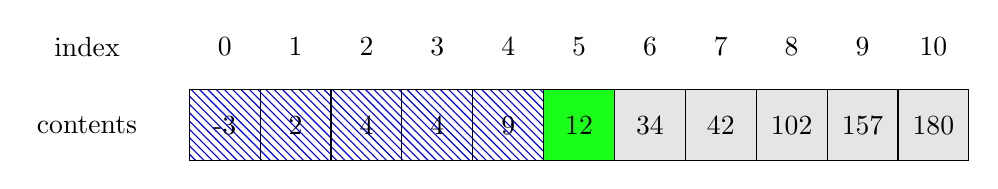
\begin{tikzpicture}
% size of each node
\def\sz{9mm}
% node style definition
\tikzstyle{block} = [
	draw, fill=black!10, rectangle,
	minimum height=\sz, minimum width=\sz ];
\tikzstyle{plain} = [draw=none,fill=none];
% array element definition
\def\arr{0, 2, 4, 4, 9, 12, 34, 42, 102};
%\def\x{0}; % x pos of arr
%\def\y{0}; % y pos of arr
%\newcounter{ind};
%\setcounter{ind}{0};
\node[plain] at (-1.75, 1) { index };
\node[plain] at (-1.75, 0) { contents };

\node[block,pattern=north west lines, pattern color=blue] at (0,0) { -3 };
\node[plain] at (0,1.0) { 0 };

\node[block,pattern=north west lines, pattern color=blue] at (1*\sz,0) { 2 };
\node[plain] at (1*\sz,1.0) { 1 };

\node[block,pattern=north west lines, pattern color=blue] at (2*\sz,0) { 4 };
\node[plain] at (2*\sz,1.0) { 2 };

\node[block,pattern=north west lines, pattern color=blue] at (3*\sz,0) { 4 };
\node[plain] at (3*\sz,1.0) { 3 };

\node[block,pattern=north west lines, pattern color=blue] at (4*\sz,0) { 9 };
\node[plain] at (4*\sz,1.0) { 4 };

\node[block,fill=white!10!green] at (5*\sz,0) { 12 };
\node[plain] at (5*\sz,1.0) { 5 };

\node[block] at (6*\sz,0) { 34 };
\node[plain] at (6*\sz,1.0) { 6 };

\node[block] at (7*\sz,0) { 42 };
\node[plain] at (7*\sz,1.0) { 7 };

\node[block] at (8*\sz,0) { 102 };
\node[plain] at (8*\sz,1.0) { 8 };

\node[block] at (9*\sz,0) { 157 };
\node[plain] at (9*\sz,1.0) { 9 };

\node[block] at (10*\sz,0) { 180 };
\node[plain] at (10*\sz,1.0) { 10 };

\end{tikzpicture}
\end{center}

\end{frame}

\begin{frame}[fragile]
  \frametitle{Example}
  \framesubtitle{}%3

~
$$l = 6, \quad r = 10, \quad m = 8$$

\begin{center}
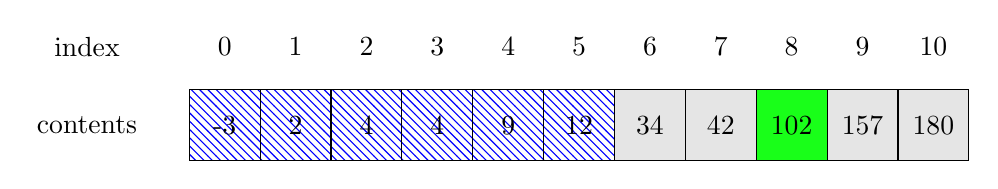
\begin{tikzpicture}
% size of each node
\def\sz{9mm}
% node style definition
\tikzstyle{block} = [
	draw, fill=black!10, rectangle,
	minimum height=\sz, minimum width=\sz ];
\tikzstyle{plain} = [draw=none,fill=none];
% array element definition
\def\arr{0, 2, 4, 4, 9, 12, 34, 42, 102};
%\def\x{0}; % x pos of arr
%\def\y{0}; % y pos of arr
%\newcounter{ind};
%\setcounter{ind}{0};
\node[plain] at (-1.75, 1) { index };
\node[plain] at (-1.75, 0) { contents };

\node[block,pattern=north west lines, pattern color=blue] at (0,0) { -3 };
\node[plain] at (0,1.0) { 0 };

\node[block,pattern=north west lines, pattern color=blue] at (1*\sz,0) { 2 };
\node[plain] at (1*\sz,1.0) { 1 };

\node[block,pattern=north west lines, pattern color=blue] at (2*\sz,0) { 4 };
\node[plain] at (2*\sz,1.0) { 2 };

\node[block,pattern=north west lines, pattern color=blue] at (3*\sz,0) { 4 };
\node[plain] at (3*\sz,1.0) { 3 };

\node[block,pattern=north west lines, pattern color=blue] at (4*\sz,0) { 9 };
\node[plain] at (4*\sz,1.0) { 4 };

\node[block,pattern=north west lines, pattern color=blue] at (5*\sz,0) { 12 };
\node[plain] at (5*\sz,1.0) { 5 };

\node[block] at (6*\sz,0) { 34 };
\node[plain] at (6*\sz,1.0) { 6 };

\node[block] at (7*\sz,0) { 42 };
\node[plain] at (7*\sz,1.0) { 7 };

\node[block] at (8*\sz,0) { 102 };
\onslide<2->{\node[block,fill=white!10!green] at (8*\sz,0) { 102 };}

\node[plain] at (8*\sz,1.0) { 8 };

\node[block] at (9*\sz,0) { 157 };
\node[plain] at (9*\sz,1.0) { 9 };

\node[block] at (10*\sz,0) { 180 };
\node[plain] at (10*\sz,1.0) { 10 };

\end{tikzpicture}
\end{center}

\end{frame}

\begin{frame}[fragile]
  \frametitle{Example}
  \framesubtitle{}%4

$42 < 102$:
$$l = 6, \quad r = 7, \quad m = 8$$
  
\begin{center}
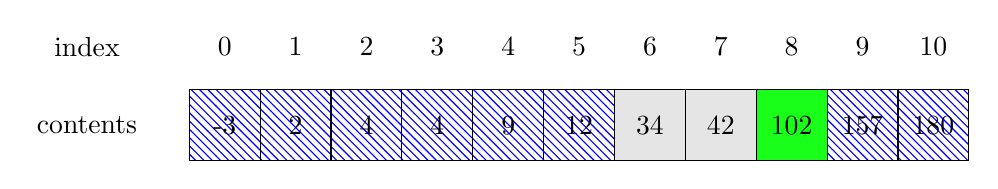
\begin{tikzpicture}
% size of each node
\def\sz{9mm}
% node style definition
\tikzstyle{block} = [
	draw, fill=black!10, rectangle,
	minimum height=\sz, minimum width=\sz ];
\tikzstyle{plain} = [draw=none,fill=none];
% array element definition
\def\arr{0, 2, 4, 4, 9, 12, 34, 42, 102};
%\def\x{0}; % x pos of arr
%\def\y{0}; % y pos of arr
%\newcounter{ind};
%\setcounter{ind}{0};
\node[plain] at (-1.75, 1) { index };
\node[plain] at (-1.75, 0) { contents };

\node[block,pattern=north west lines, pattern color=blue] at (0,0) { -3 };
\node[plain] at (0,1.0) { 0 };

\node[block,pattern=north west lines, pattern color=blue] at (1*\sz,0) { 2 };
\node[plain] at (1*\sz,1.0) { 1 };

\node[block,pattern=north west lines, pattern color=blue] at (2*\sz,0) { 4 };
\node[plain] at (2*\sz,1.0) { 2 };

\node[block,pattern=north west lines, pattern color=blue] at (3*\sz,0) { 4 };
\node[plain] at (3*\sz,1.0) { 3 };

\node[block,pattern=north west lines, pattern color=blue] at (4*\sz,0) { 9 };
\node[plain] at (4*\sz,1.0) { 4 };

\node[block,pattern=north west lines, pattern color=blue] at (5*\sz,0) { 12 };
\node[plain] at (5*\sz,1.0) { 5 };

\node[block] at (6*\sz,0) { 34 };
\node[plain] at (6*\sz,1.0) { 6 };

\node[block] at (7*\sz,0) { 42 };
\node[plain] at (7*\sz,1.0) { 7 };

\node[block,fill=white!10!green] at (8*\sz,0) { 102 };
\node[plain] at (8*\sz,1.0) { 8 };

\node[block,pattern=north west lines, pattern color=blue] at (9*\sz,0) { 157 };
\node[plain] at (9*\sz,1.0) { 9 };

\node[block,pattern=north west lines, pattern color=blue] at (10*\sz,0) { 180 };
\node[plain] at (10*\sz,1.0) { 10 };

\end{tikzpicture}
\end{center}

\end{frame}

\begin{frame}[fragile]
  \frametitle{Example}
  \framesubtitle{}%5

\onslide<2->{
  $34 < 42 = k$:
}
$$l = 6, \quad r = 7, \quad m = 6$$
\begin{center}  
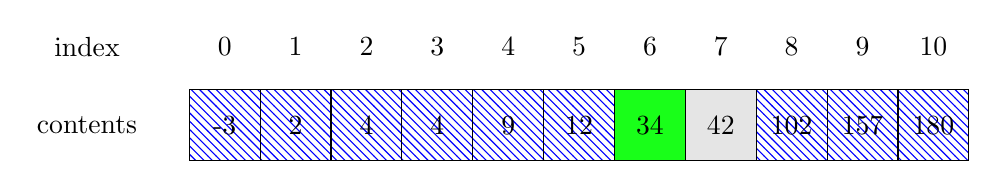
\begin{tikzpicture}
% size of each node
\def\sz{9mm}
% node style definition
\tikzstyle{block} = [
	draw, fill=black!10, rectangle,
	minimum height=\sz, minimum width=\sz ];
\tikzstyle{plain} = [draw=none,fill=none];
% array element definition
\def\arr{0, 2, 4, 4, 9, 12, 34, 42, 102};
%\def\x{0}; % x pos of arr
%\def\y{0}; % y pos of arr
%\newcounter{ind};
%\setcounter{ind}{0};
\node[plain] at (-1.75, 1) { index };
\node[plain] at (-1.75, 0) { contents };

\node[block,pattern=north west lines, pattern color=blue] at (0,0) { -3 };
\node[plain] at (0,1.0) { 0 };

\node[block,pattern=north west lines, pattern color=blue] at (1*\sz,0) { 2 };
\node[plain] at (1*\sz,1.0) { 1 };

\node[block,pattern=north west lines, pattern color=blue] at (2*\sz,0) { 4 };
\node[plain] at (2*\sz,1.0) { 2 };

\node[block,pattern=north west lines, pattern color=blue] at (3*\sz,0) { 4 };
\node[plain] at (3*\sz,1.0) { 3 };

\node[block,pattern=north west lines, pattern color=blue] at (4*\sz,0) { 9 };
\node[plain] at (4*\sz,1.0) { 4 };

\node[block,pattern=north west lines, pattern color=blue] at (5*\sz,0) { 12 };
\node[plain] at (5*\sz,1.0) { 5 };

\node[block] at (6*\sz,0) { 34 };
\onslide<2->{
\node[block,fill=white!10!green] at (6*\sz,0) { 34 };
}
\node[plain] at (6*\sz,1.0) { 6 };

\node[block] at (7*\sz,0) { 42 };
\node[plain] at (7*\sz,1.0) { 7 };

\node[block,pattern=north west lines, pattern color=blue] at (8*\sz,0) { 102 };
\node[plain] at (8*\sz,1.0) { 8 };

\node[block,pattern=north west lines, pattern color=blue] at (9*\sz,0) { 157 };
\node[plain] at (9*\sz,1.0) { 9 };

\node[block,pattern=north west lines, pattern color=blue] at (10*\sz,0) { 180 };
\node[plain] at (10*\sz,1.0) { 10 };

\end{tikzpicture}

\end{center}

\end{frame}

\begin{frame}[fragile]
  \frametitle{Example}
  \framesubtitle{}%6
  
\onslide<2->{
$a_7 = 42 = k$}
$$l = 7, \quad r = 7, \quad m = 7$$

\begin{center}
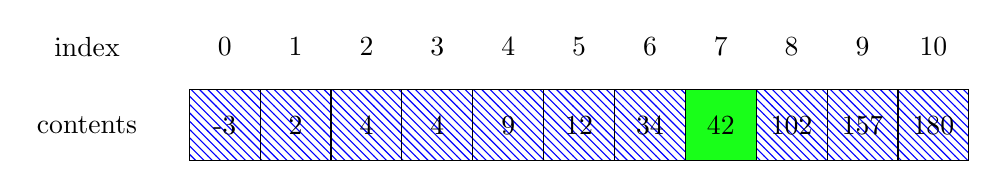
\begin{tikzpicture}
% size of each node
\def\sz{9mm}
% node style definition
\tikzstyle{block} = [
	draw, fill=black!10, rectangle,
	minimum height=\sz, minimum width=\sz ];
\tikzstyle{plain} = [draw=none,fill=none];
% array element definition
\def\arr{0, 2, 4, 4, 9, 12, 34, 42, 102};
%\def\x{0}; % x pos of arr
%\def\y{0}; % y pos of arr
%\newcounter{ind};
%\setcounter{ind}{0};
\node[plain] at (-1.75, 1) { index };
\node[plain] at (-1.75, 0) { contents };

\node[block,pattern=north west lines, pattern color=blue] at (0,0) { -3 };
\node[plain] at (0,1.0) { 0 };

\node[block,pattern=north west lines, pattern color=blue] at (1*\sz,0) { 2 };
\node[plain] at (1*\sz,1.0) { 1 };

\node[block,pattern=north west lines, pattern color=blue] at (2*\sz,0) { 4 };
\node[plain] at (2*\sz,1.0) { 2 };

\node[block,pattern=north west lines, pattern color=blue] at (3*\sz,0) { 4 };
\node[plain] at (3*\sz,1.0) { 3 };

\node[block,pattern=north west lines, pattern color=blue] at (4*\sz,0) { 9 };
\node[plain] at (4*\sz,1.0) { 4 };

\node[block,pattern=north west lines, pattern color=blue] at (5*\sz,0) { 12 };
\node[plain] at (5*\sz,1.0) { 5 };

\node[block,pattern=north west lines, pattern color=blue] at (6*\sz,0) { 34 };
\node[plain] at (6*\sz,1.0) { 6 };

\node[block,fill=white!10!green] at (7*\sz,0) { 42 };
\node[plain] at (7*\sz,1.0) { 7 };

\node[block,pattern=north west lines, pattern color=blue] at (8*\sz,0) { 102 };
\node[plain] at (8*\sz,1.0) { 8 };

\node[block,pattern=north west lines, pattern color=blue] at (9*\sz,0) { 157 };
\node[plain] at (9*\sz,1.0) { 9 };

\node[block,pattern=north west lines, pattern color=blue] at (10*\sz,0) { 180 };
\node[plain] at (10*\sz,1.0) { 10 };

\end{tikzpicture}

\end{center}

\end{frame}

\begin{frame}[fragile]
  \frametitle{Recursive Code}
  \framesubtitle{}

\begin{minted}{c}
int binarySearch(const int *arr, int l, int r, int k) {
  if(l > r) {
    return -1;
  } else {
    int m = (l + r) / 2; //bad in practice
    
    if(arr[m] == k) {
      return m;
    } else if(k < arr[m]) {
      return binarySearch(arr, l, m-1, k);
    } else if(arr[m] < k) {
      return binarySearch(arr, m+1, r, k);
    }
  }
}
\end{minted}

\end{frame}

\begin{frame}[fragile]
  \frametitle{Iterative Code}
  \framesubtitle{}

\begin{minted}{c}
int binarySearch(const int *arr, int n, int k) {
  int l = 0;
  int r = n-1;
  while(l <= r) {
    int m = (l + r) / 2; //bad in practice
    
    if(arr[m] == k) {
      return m;
    } else if(k < arr[m]) {
      r = m - 1;
    } else if(arr[m] < k) {
      l = m+1;
    }
  }
  return -1;
}
\end{minted}

\end{frame}

\subsection{Analysis}

\begin{frame}[fragile]
  \frametitle{Analysis}
  \framesubtitle{}


\begin{itemize}[<+->]
  \item Which is better?  How much better?
  \item How much ``work'' does each algorithm perform?
  \item Suppose we search an array of $n$ elements
  \item How many \emph{comparisons} does each search perform?
\end{itemize}

\end{frame}


\begin{frame}[fragile]
  \frametitle{Linear Search Analysis}
  \framesubtitle{}
  
\begin{itemize}[<+->]
  \item Best case scenario: you get lucky and immediately find the element, making one single comparison
  \item Worst Case: you are unlucky and make all $n$ comparisons
  \item Average case scenario: $\approx \frac{n}{2}$ comparisons
  \item Called \emph{linear search} because the work is \emph{linearly} proportional to the array size
\end{itemize}

\end{frame}

\begin{frame}[fragile]
  \frametitle{Binary Search}
  \framesubtitle{}
  
\begin{itemize}[<+->]
  \item Worst case scenario: unsuccessful search
  \item Or: when the list size is cut down to size 1
  \item Each comparison cuts the array (roughly) in half
  \item After first iteration:
  	$$\frac{n}{2}$$
  \item After second:	
  	$$\frac{n}{4}$$
\end{itemize}
\end{frame}

\begin{frame}[fragile]
  \frametitle{Binary Search}
  \framesubtitle{}
  
\begin{itemize}[<+->]
    \item After third:	
  	$$\frac{n}{8}$$
  \item After $k$ iterations:	
  	$$\frac{n}{2^k}$$
  \item Stops when 
  	$$\frac{n}{2^k} = 1$$
  \item Solve for $k$: 
    $$k = \log_2{(n)}$$    
  \item Roughly only $\log_2{(n)}$ comparisons are made.
\end{itemize}

\end{frame}

\begin{frame}[fragile]
  \frametitle{Comparison}
  \framesubtitle{}

\begin{itemize}[<+->]
  \item Linear: $\approx n$ versus Binary Search: $\log_2{(n)}$
  \item Linear search is \emph{exponentially worse}
  \item Binary search is \emph{exponentially faster}
\end{itemize}

\end{frame}

\begin{frame}[fragile]
  \frametitle{Perspective}
  \framesubtitle{}

\begin{itemize}[<+->]
  \item Suppose we have a database of 1 trillion, $10^{12}$ elements
  \item Unsorted using linear search: 
    $$\approx 5\times 10^{11}$$
    comparisons
  \item Sorted (``indexed'') using binary search:
    $$\approx \log_2{(10^{12})} \approx 40$$
    comparisons
\end{itemize}

\end{frame}

\begin{frame}[fragile]
  \frametitle{Another Perspective}
  \framesubtitle{Growth Rate}

\begin{itemize}[<+->]
  \item Suppose we \emph{double} the input size: $n \rightarrow 2n$
  \item Linear search would require $n \rightarrow 2n$ comparisons
  \item Doubling the input size doubles the number of comparisons
  \item Binary search: 
   $$\log_2{(n)} \rightarrow \log_2{(2n)}$$
  \item $\log_2{(2n)} = \log_2{(n)} + 1$
  \item Doubling the input size only adds one more comparison!
\end{itemize}

\end{frame}

\section{Selection Sort}

\begin{frame}
    \frametitle{}
    \framesubtitle{}
    
    \begin{center}
    {\Huge Part III: Selection Sort}\\
    {\Large ~}
    \end{center}

\end{frame}

\begin{frame}[fragile]
  \frametitle{Introduction}
  \framesubtitle{}

\begin{itemize}[<+->]
  \item To exploit binary search we need to be able to sort
  \item Many different sorting algorithms each with different properites
  \item Bubble Sort, Selection Sort, Insertion Sort, Quick Sort, Merge Sort, 
  Heap Sort, Tim Sort, etc.
  \item Some efficient, some inefficient
  \item Start with a simple implementation: Selection Sort 
\end{itemize} 

\end{frame}

\begin{frame}[fragile]
  \frametitle{Basic Idea}
  \framesubtitle{} 
  
\begin{itemize}[<+->]
  \item Search through the array and find the minimal element
  \item Swap it with the first element
  \item Proceed with the remainder of the array
  \item In general: 
  \begin{itemize}
    \item $i$-th iteration: find minimal element in \mintinline{c}{arr[i]} through
     \mintinline{c}{arr[n-1]}
    \item Swap it with \mintinline{c}{arr[i]}
    \item Stop at $i=n-1$ (last element is already sorted)
  \end{itemize}
  \item Demonstration
\end{itemize}
  
\end{frame}

\begin{frame}[fragile]
  \frametitle{Selection Sort Example}
  \framesubtitle{Iteration 1}

\begin{center}
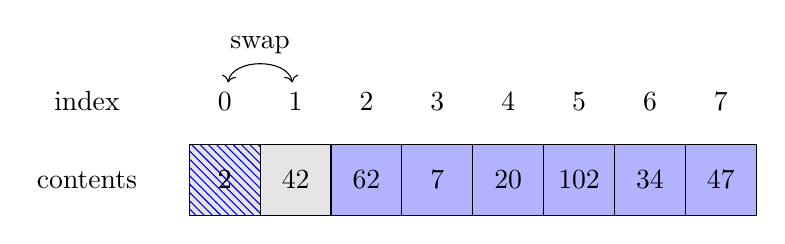
\begin{tikzpicture}
% size of each node
\def\sz{9mm}
% node style definition
\tikzstyle{block} = [
	draw, fill=black!10, rectangle,
	minimum height=\sz, minimum width=\sz ];
\tikzstyle{plain} = [draw=none,fill=none];


%pattern=north west lines, pattern color=blue

\node[plain] at (-1.75, 1) { index };
\node[plain] at (-1.75, 0) { contents };

\node[block] at (0,0) { 42 };
\onslide<2-3>{\node[block,fill=white!50!blue] (a42) at (0,0) { 42 };}
\onslide<12->{\node[block]  at (0,0) { 2 };}
\onslide<13>{\node[block,pattern=north west lines, pattern color=blue]  at (0,0) { 2 };}
\node[plain] (X) at (0,1.0) { 0 };

\node[block] at (1*\sz,0) { 2 };
\onslide<3>{
  \node[block,fill=white!70!blue] (a2) at (1*\sz,0) { 2 };
}
\onslide<4->{
  \node[block,fill=white!50!blue] at (1*\sz,0) { 2 };
}
\node[plain] (Y) at (1*\sz,1.0) { 1 };
\onslide<12->{\node[block]  at (1*\sz,0) { 42 };}

\node[block] at (2*\sz,0) { 62 };
\onslide<5>{\node[block,fill=white!70!blue] (a62) at (2*\sz,0) { 62 };}
\node[plain] at (2*\sz,1.0) { 2 };

\node[block] at (3*\sz,0) { 7 };
\onslide<6>{\node[block,fill=white!70!blue] (a7) at (3*\sz,0) { 7 };}
\node[plain] at (3*\sz,1.0) { 3 };

\node[block] at (4*\sz,0) { 20 };
\onslide<7>{\node[block,fill=white!70!blue] (a20) at (4*\sz,0) { 20 };}
\node[plain] at (4*\sz,1.0) { 4 };

\node[block] at (5*\sz,0) { 102 };
\onslide<8>{\node[block,fill=white!70!blue] (a102) at (5*\sz,0) { 102 };}
\node[plain] at (5*\sz,1.0) { 5 };

\node[block] at (6*\sz,0) { 34 };
\onslide<9>{\node[block,fill=white!70!blue] (a34) at (6*\sz,0) { 34 };}
\node[plain] at (6*\sz,1.0) { 6 };

\node[block] at (7*\sz,0) { 47 };
\onslide<10>{\node[block,fill=white!70!blue] (a47) at (7*\sz,0) { 47 };}
\node[plain] at (7*\sz,1.0) { 7 };

\onslide<11>{
  \draw[<->,out=80,in=100] (X) edge node[pos=.5,above] {swap} (Y);
}

\end{tikzpicture}
\end{center}

\end{frame}

\begin{frame}[fragile]
  \frametitle{Selection Sort Example}
  \framesubtitle{Iteration 2}

\begin{center}
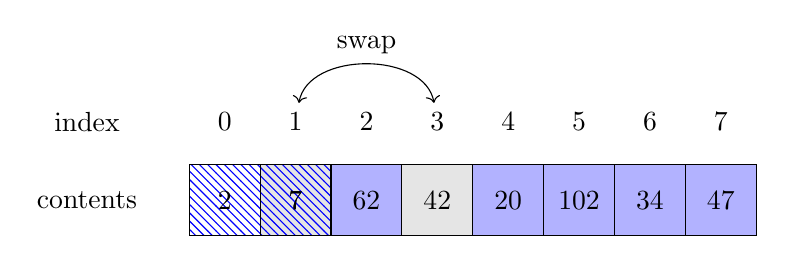
\begin{tikzpicture}
% size of each node
\def\sz{9mm}
% node style definition
\tikzstyle{block} = [
	draw, fill=black!10, rectangle,
	minimum height=\sz, minimum width=\sz ];
\tikzstyle{plain} = [draw=none,fill=none];


%pattern=north west lines, pattern color=blue

\node[plain] at (-1.75, 1) { index };
\node[plain] at (-1.75, 0) { contents };

\node[block,pattern=north west lines, pattern color=blue] at (0,0) { 2 };
\node[plain] (X) at (0,1.0) { 0 };

\node[block] at (1*\sz,0) { 42 };
\onslide<2-4>{
  \node[block,fill=white!50!blue] (a2) at (1*\sz,0) { 42 };
}
\onslide<12->{
  \node[block] at (1*\sz,0) { 7 };
}
\onslide<13->{
  \node[block,pattern=north west lines, pattern color=blue] at (1*\sz,0) { 7 };
}
\node[plain] (Y) at (1*\sz,1.0) { 1 };

\node[block] at (2*\sz,0) { 62 };
\onslide<3>{\node[block,fill=white!70!blue] (a62) at (2*\sz,0) { 62 };}
\node[plain] at (2*\sz,1.0) { 2 };

\node[block] at (3*\sz,0) { 7 };
\onslide<4>{\node[block,fill=white!70!blue] (a7) at (3*\sz,0) { 7 };}
\onslide<5->{\node[block,fill=white!50!blue] (a7) at (3*\sz,0) { 7 };}
\onslide<12->{
  \node[block] at (3*\sz,0) { 42 };
}
\node[plain] (Z) at (3*\sz,1.0) { 3 };

\node[block] at (4*\sz,0) { 20 };
\onslide<6>{\node[block,fill=white!70!blue] (a20) at (4*\sz,0) { 20 };}
\node[plain] at (4*\sz,1.0) { 4 };

\node[block] at (5*\sz,0) { 102 };
\onslide<7>{\node[block,fill=white!70!blue] (a102) at (5*\sz,0) { 102 };}
\node[plain] at (5*\sz,1.0) { 5 };

\node[block] at (6*\sz,0) { 34 };
\onslide<8>{\node[block,fill=white!70!blue] (a34) at (6*\sz,0) { 34 };}
\node[plain] at (6*\sz,1.0) { 6 };

\node[block] at (7*\sz,0) { 47 };
\onslide<9>{\node[block,fill=white!70!blue] (a47) at (7*\sz,0) { 47 };}
\node[plain] at (7*\sz,1.0) { 7 };

\onslide<11>{
  \draw[<->,out=80,in=100] (Y) edge node[pos=.5,above] {swap} (Z);
}

\end{tikzpicture}
\end{center}

\end{frame}

\begin{frame}[fragile]
  \frametitle{}
  \framesubtitle{}

\begin{minted}{c}
void selectionSort(int *arr, int n) {

  for(int i=0; i<n-1; i++) {
    int minIndex = i;
    for(int j=i+1; j<n; j++) {
      if(arr[j] < arr[minIndex]) {
        minIndex = j;
      }
    }
    //swap
    int temp = arr[i];
    arr[i] = arr[minIndex];
    arr[minIndex] = temp;
  }
}
\end{minted}
  
\end{frame}

\begin{frame}[fragile]
  \frametitle{Analysis}
  \framesubtitle{} 
  
\begin{itemize}[<+->]
  \item Selection sort is simple, but naive and inefficient
  \item How bad is it?
  \item How many comparisons does selection sort make on an array of size $n$?
  \begin{itemize}
    \item First iteration: $n-1$ comparisons 
    \item Second iteration: $n-2$ comparisons
    \item $i$-th iteration: $n-i$ comparisons
    \item Last iteration: 1 comparison
    \item In total: 
      $$1 + 2 + 3 + \cdots + (n-2) + (n-1) = \frac{n(n-1)}{2} = \frac{1}{2}n^2 + \frac{1}{2}n$$
  \end{itemize}
\end{itemize}
\end{frame}

\begin{frame}[fragile]
  \frametitle{Perspective}
  \framesubtitle{} 
  
\begin{itemize}[<+->]
  \item Selection sort is a \emph{quadratic}, $\approx n^2$ sorting algorithm
  \item How bad is this?
  \item Sorting the database of 1 trillion, $10^{12}$ elements requires
    $$\approx 5 \times 10^{23}$$
  \item 500 ``Sextillion'' comparisons
  \item NVIDIA GTX 1080Ti: 11.3 TeraFLOPS
  \item[~]
    $$\frac{5 * 10^{23} \textrm{ operations}}{11.3 * 10^{12} \textrm{ ops/sec}} = 1,402.157 \textbf{ years}$$
  \item Not feasible for even ``moderately large'' inputs
\end{itemize}

\end{frame}

\begin{frame}[fragile]
  \frametitle{Another Perspective}
  \framesubtitle{} 
  
\begin{itemize}[<+->]
  \item Double the size of the array: $n \rightarrow 2n$
  \item Number of comparisons grows:
  	$$n^2 \rightarrow (2n)^2 = 4n^2$$
  \item Doubling the input \emph{quadruples} the number of operations
  \item Four times slower!
\end{itemize}
  
\end{frame}


\section{Quick Sort}

\begin{frame}
    \frametitle{}
    \framesubtitle{}
    
    \begin{center}
    {\Huge Part IV: Quick Sort}\\
    {\Large ~}
    \end{center}

\end{frame}

\begin{frame}[fragile]
  \frametitle{}
  \framesubtitle{}

\begin{itemize}[<+->]
  \item We need a better, more efficient sorting algorithm
  \item Lots exist, focus on Quick Sort
  \item High level description only
  \item Many variations of the same idea
  \item Basic Divide \& Conquer strategy
\end{itemize}

\end{frame}

\begin{frame}[fragile]
  \frametitle{Basic Idea}
  \framesubtitle{}

\begin{itemize}[<+->]
  \item Choose a \emph{pivot} element
  \item Partition elements around this pivot
  \item Smaller elements to the left
  \item Larger elements to the right
  \item Place the pivot in the middle
  \item Pivot ends up where it should be
  \item Recursively run quick sort on the left and right halves
  \item Demonstration
\end{itemize}

\end{frame}

\begin{frame}[fragile]
  \frametitle{Quick Sort Example}
  \framesubtitle{}
  
\begin{center}
\begin{tikzpicture}
% size of each node
\def\sz{9mm}
% node style definition
\tikzstyle{block} = [
	draw, fill=black!10, rectangle,
	minimum height=\sz, minimum width=\sz ];
\tikzstyle{plain} = [draw=none,fill=none];
% array element definition
\def\arr{0, 2, 4, 4, 9, 12, 34, 42, 102};
%\def\x{0}; % x pos of arr
%\def\y{0}; % y pos of arr
%\newcounter{ind};
%\setcounter{ind}{0};
\node[plain] at (-1.75, 1) { index };
\node[plain] at (-1.75, 0) { contents };

\node[block] at (0,0) { 42 };
\onslide<2->{\node[block,fill=white!50!green] (a42) at (0,0) { 42 };}
\node[plain] at (0,1.0) { 0 };

\node[block] at (1*\sz,0) { 2 };
\onslide<3>{
  \node[block,fill=white!70!blue] (a2) at (1*\sz,0) { 2 };
}
\node[plain] at (1*\sz,1.0) { 1 };

\node[block] at (2*\sz,0) { 62 };
\onslide<4>{\node[block,fill=white!70!blue] (a62) at (2*\sz,0) { 62 };}
\node[plain] at (2*\sz,1.0) { 2 };

\node[block] at (3*\sz,0) { 7 };
\onslide<5>{\node[block,fill=white!70!blue] (a7) at (3*\sz,0) { 7 };}
\node[plain] at (3*\sz,1.0) { 3 };

\node[block] at (4*\sz,0) { 20 };
\onslide<6>{\node[block,fill=white!70!blue] (a20) at (4*\sz,0) { 20 };}
\node[plain] at (4*\sz,1.0) { 4 };

\node[block] at (5*\sz,0) { 102 };
\onslide<7>{\node[block,fill=white!70!blue] (a102) at (5*\sz,0) { 102 };}
\node[plain] at (5*\sz,1.0) { 5 };

\node[block] at (6*\sz,0) { 34 };
\onslide<8>{\node[block,fill=white!70!blue] (a34) at (6*\sz,0) { 34 };}
\node[plain] at (6*\sz,1.0) { 6 };

\node[block] at (7*\sz,0) { 47 };
\onslide<9>{\node[block,fill=white!70!blue] (a47) at (7*\sz,0) { 47 };}
\node[plain] at (7*\sz,1.0) { 7 };


\node[plain] at (-1.75, -3) {$pivot = 42$ };

\node[block] at (0,-3) { ~ };
\onslide<3->{
  \node[block] (b2) at (0,-3) { 2 };
}
\onslide<3>{
  \draw[->] (a2) |- (0,-1.5) -| (b2.north);
}

\node[block] at (1*\sz,-3) { ~ };
\onslide<5->{
  \node[block] (b7) at (1*\sz,-3) { 7 };
}
\onslide<5>{
  \draw[->] (a7) |- (1,-1.5) -| (b7.north);
}

\node[block] at (2*\sz,-3) { ~ };
\onslide<6->{
  \node[block] (b20) at (2*\sz,-3) { 20 };
}
\onslide<6>{
  \draw[->] (a20) |- (2,-1.5) -| (b20.north);
}

\node[block] at (3*\sz,-3) { ~ };
\onslide<8->{
  \node[block] (b34) at (3*\sz,-3) { 34 };
}
\onslide<8>{
  \draw[->] (a34) |- (3,-1.5) -| (b34.north);
}


\node[block] at (4*\sz,-3) { ~ };
\onslide<10->{
  \node[block,fill=white!50!black] (b42) at (4*\sz,-3) { 42 };
}
\onslide<10>{
  \draw[->] (a42) |- (3,-1.5) -| (b42.north);
}


\node[block] at (5*\sz,-3) { ~ };
\onslide<9->{
  \node[block] (b47) at (5*\sz,-3) { 47 };
}
\onslide<9>{
  \draw[->] (a47) |- (5,-1.5) -| (b47.north);
}


\node[block] at (6*\sz,-3) { ~ };
\onslide<7->{
  \node[block] (b102) at (6*\sz,-3) { 102 };
}
\onslide<7>{
  \draw[->] (a102) |- (5,-1.5) -|(b102.north);
}


\node[block] at (7*\sz,-3) { ~ };
\onslide<4->{
\node[block] (b62) at (7*\sz,-3) { 62 };
}
\onslide<4>{
  \draw[->] (a62) |- (6,-1.5) -| (b62.north);
}

\onslide<11>{
  \node (left)  at (1.5*\sz,-4.5) {\mintinline{c}{quickSort(arr, 0, 3);}};
  \node (right) at (6.5*\sz,-4.5) {\mintinline{c}{quickSort(arr, 5, 7);}};
}

\end{tikzpicture}

\end{center}

\end{frame}

\begin{frame}[fragile]
  \frametitle{Analysis}
  \framesubtitle{}


\begin{itemize}[<+->]
  \item Best/Worst/Average case analysis
  \item Quick Sort makes roughly $n \log_2{(n)}$ comparisons
  \item \emph{Much} better than $n^2$
  \item Comparisons
\end{itemize}

\end{frame}

\begin{frame}[fragile]
  \frametitle{Analysis}
  \framesubtitle{}

\begin{itemize}[<+->]
  \item Sorting the database of 1 trillion, $10^{12}$ records
  \item Comparisons:
    $$10^{12} \cdot \log_2{10^{12}} \approx 4 \times 10^{13}$$
  \item 40 trillion comparisons
  \item NVIDIA GTX 1080Ti: 11.3 TeraFLOPS
  \item[~]
    $$\frac{4 \times 10^{13} \textrm{ operations}}{11.3 * 10^{12} \textrm{ ops/sec}} = 3.5 \textbf{ seconds}$$
  \item Very feasible
\end{itemize}  
  
\end{frame}

\begin{frame}[fragile]
  \frametitle{Analysis}
  \framesubtitle{}  

\begin{itemize}[<+->]
  \item Consider doubling the input size: $n \rightarrow 2n$
  \item Number of comparisons:
   $$n\log_2{(n)} \rightarrow 2n\log_2{(2n)}$$
  \item $2n\log_2{(2n)} = 2n\log_2{(n)} + 2n$
  \item Roughly only twice as many
  \item Often referred to as \emph{quasilinear}
\end{itemize}

\end{frame}

\section{Sorting in Practice}

\begin{frame}
    \frametitle{}
    \framesubtitle{}
    
    \begin{center}
    {\Huge Part V: Sorting in Practice}\\
    {\Large ~}
    \end{center}

\end{frame}

\begin{frame}[fragile]
  \frametitle{In Practice}
  \framesubtitle{}

\begin{itemize}[<+->]
  \item Don't ``roll your own'' searching/sorting algorithms
  \item Use standard library functions
  \item \emph{But}: we don't want dozens of different functions one for each type of variable or criteria that we want to sort with respect to
  \item Want ONE generic solution that can sort \emph{any} type of 
  data by \emph{any} criteria
  \item One sorting function to sort them all
\end{itemize}

\end{frame}

\subsection{Comparators}

\begin{frame}[fragile]
  \frametitle{Comparators}
  \framesubtitle{}

\begin{itemize}[<+->]
  \item Solution: use one \emph{generic} sorting function 
  \item Needs to know how to order two elements, $a, b$
  \item Are they in order or do they need to be swapped?
  \item Solution: A \emph{comparator} function
  \item Given two elements $a, b$ it returns:
  \begin{itemize}
     \item \emph{something} negative if $a < b$
     \item zero if $a=b$
     \item \emph{something} positive if $a>b$
  \end{itemize}
\end{itemize}

\end{frame}

\begin{frame}[fragile]
  \frametitle{Comparator Illustration}
  \framesubtitle{}
  
\begin{center}
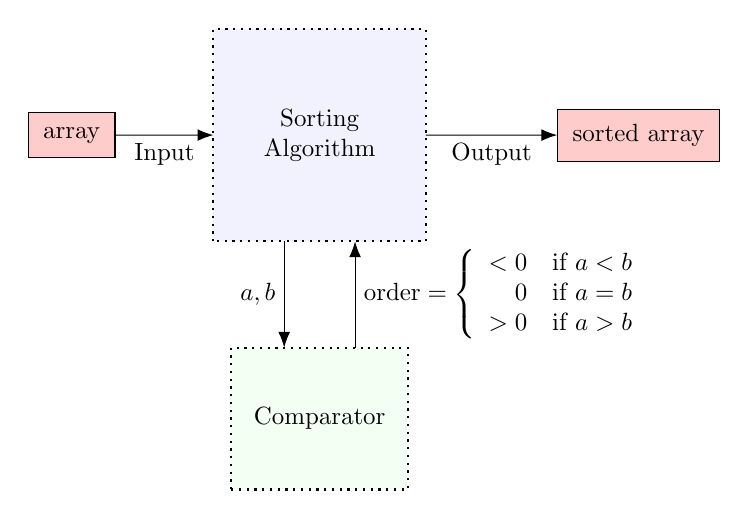
\begin{tikzpicture}[scale=.90,transform shape,
fringeedge/.style={green!50!yellow!50!black,thick},
edge/.style={->,thick},
place/.style={rectangle,draw=black,fill=red!20,inner sep=6pt,minimum size=6mm},
transition/.style={rectangle,draw=black!50,fill=black!20,thick,inner sep=0pt,minimum size=4mm}] 

\draw[fill=blue!5,thick,dotted] (0,0) rectangle (3,3);
\node[] at (1.5,1.5) {
\begin{tabular}{c}
Sorting \\
Algorithm
\end{tabular}
};

\node (INPUT) at (-2,1.5) [place] {array};
\draw[-{Latex[length=2mm]}] (INPUT) -- node[pos=.5,below] {Input} (0, 1.5);

\node (OUTPUT) at (6,1.5) [place] {sorted array};
\draw[-{Latex[length=2mm]}] (3,1.5) -- node[pos=.5,below] {Output} (OUTPUT);

\draw[fill=green!5,thick,dotted] (.25,-3.5) rectangle (2.75,-1.5);
\node[] at (1.5,-2.5) {Comparator};


\draw[-{Latex[length=2mm]}] (1,0) -- node[left,pos=.5] {$a, b$} (1,-1.5);

\draw[{Latex[length=2mm]}-] (2,0) -- node[right,pos=.5] {
$\textrm{order} = \left\{
\begin{array}{rl}
< 0 & \textrm{if } a < b \\
0 & \textrm{if } a = b \\
> 0 & \textrm{if } a > b
\end{array}\right.$} (2,-1.5);

\end{tikzpicture}
\end{center}

\end{frame}

\subsection{Comparators in C}


\begin{frame}[fragile]
  \frametitle{Comparators in C}
  \framesubtitle{}

\begin{itemize}[<+->]
  \item In C, a \emph{comparator function} has the following signature
  \item \mintinline{c}{int cmp(const void *a, const void *b);}
  \item \mintinline{c}{const} means we won't change it, only compare it
  \item \mintinline{c}{void *} is a \emph{generic pointer} that can point
  to anything
  \item Recall: \mintinline{c}{malloc()}
\end{itemize}

\end{frame}

\begin{frame}[fragile]
  \frametitle{Standard Pattern}
  \framesubtitle{}

Standard Pattern:
\begin{itemize}[<+->]
  \item Cast the \mintinline{c}{void *} to a particular data type
  \item Use the data's \emph{state} to determine the proper order
  \item Return an integer value that expresses the proper order 
\end{itemize}

\end{frame}

\begin{frame}[fragile]
  \frametitle{Best Practice}
  \framesubtitle{}

Best Practices:
\begin{itemize}[<+->]
  \item Use descriptive function names
  \item Be explicit in your comparisons
  \item Avoid ``tricks''
  \item Reuse comparator functionality when possible
\end{itemize}

\end{frame}

\begin{frame}[fragile]
  \frametitle{Examples}
  \framesubtitle{}

\begin{itemize}
  \item Write a comparator to order integers in non-decreasing order
  \item Write a comparator to order integers in non-increasing order
  \item Write a comparator to order \mintinline{c}{Student} structures by NUID
  \item Write a comparator to order \mintinline{c}{Student} structures by GPA
  \item Write a comparator to order \mintinline{c}{Student} structures by last name/first name
\end{itemize}

\end{frame}

\section{Function Pointers}

\begin{frame}
    \frametitle{}
    \framesubtitle{}
    
    \begin{center}
    {\Huge Part VI: Function Pointers}\\
    {\Large ~}
    \end{center}

\end{frame}

\begin{frame}[fragile]
  \frametitle{Function Pointers}
  \framesubtitle{}

\begin{itemize}[<+->]
  \item Now that we have comparator functions: how do we pass them to a generic sorting function?
  \item Easy to pass variables by value or by reference
  \item How do we pass a function?
  \item We need \emph{function pointers}
\end{itemize}

\end{frame}

\begin{frame}[fragile]
  \frametitle{Function Pointers}
  \framesubtitle{}

\begin{itemize}[<+->]
  \item Recall: a \emph{pointer} refers to a memory location
  \item What is stored in memory? 
  \item Variables, arrays, data, \emph{everything}
  \item A program's code is stored in memory, including its \emph{functions}
  \item We can create pointers that point to memory locations that contain functions!
  \item Function pointers allow us to ``pass'' a function to another function
  \item Called ``callback'' functions
  \item Demonstration
\end{itemize}
\end{frame}

\begin{frame}[fragile]
  \frametitle{Function Pointers: Demo}
  \framesubtitle{}

\begin{minted}[fontsize=\tiny]{c}
//create a pointer called ptrToFunc that can point to a
//function that returns an integer and takes three arguments:
//(int, double, char)

int (*ptrToFunc)(int, double, char) = NULL;

//declare a pointer that can point to math's sqrt function
double (*ptrToSqrt)(double) = NULL;

//let's make ptrToSqrt point to the sqrt function
ptrToSqrt = sqrt;

//you can call a function via its pointer:
double x = ptrToSqrt(2.0);

//careful: you can reassign standard library functions:
sqrt = sin;
double y = sqrt(3.14159); //0
//don't do this

//a function that takes another function:
void runAFunction(double x, double (*func)(double)) {
  //run func on x:
  double y = func(x);  
}
\end{minted}
\end{frame}

\section{Searching \& Sorting in C}

\begin{frame}
    \frametitle{}
    \framesubtitle{}
    
    \begin{center}
    {\Huge Part VII: Searching \& Sorting in C}\\
    {\Large ~}
    \end{center}

\end{frame}

\begin{frame}[fragile]
  \frametitle{Searching \& Sorting in C}
  \framesubtitle{}

\begin{itemize}[<+->]
  \item To make generic searching \& sorting functions, we need to pass in a comparator
  \item Function pointers allow us to do this
  \item The array to be searched/sorted is also generic, \mintinline{c}{void *}
  \item Demonstration: generic linear search 
\end{itemize}

\end{frame}

\begin{frame}[fragile]
  \frametitle{Generic Linear Search}
  \framesubtitle{}

\begin{minted}[fontsize=\scriptsize]{c}
/**
 * This function takes an array of integers
 * and searches it for the given key, returning
 * the index at which it finds it, or -1 if no
 * such element exists.
 */
int linearSearch(const void *key, const void *arr, int n, int size, int (*compar) (const void *, const void *)) {

  for(int i=0; i<n; i++) {
    if(compar(key, (arr + i * size) ) == 0) {
      return i;
    }
  }
  return -1;
}
\end{minted}

\end{frame}

\begin{frame}[fragile]
  \frametitle{Sorting in C}
  \framesubtitle{}

\begin{itemize}[<+->]
  \item The standard C library provides a generic sorting function
\begin{minted}{c}
void qsort(void *base,
           size_t nel,
           size_t size,
           int (*compar)(const void *, const void *));
\end{minted}
  \item \mintinline{c}{base} is the array of elements to be sorted 
  %(also note: it is not const)
  \item \mintinline{c}{nel} is the number of elements in the array
  \item \mintinline{c}{size} is the number of bytes each element takes
  \item \mintinline{c}{compar} the comparator function you want to use to order elements
  \item Demonstration
\end{itemize}

\end{frame}

\begin{frame}[fragile]
  \frametitle{Binary Search in C}
  \framesubtitle{}

\begin{itemize}[<+->]
  \item The standard C library provides a generic binary search function
\begin{minted}{c}
void * bsearch(const void *key,
               const void *base,
               size_t nel,
               size_t size,
               int (*compar) (const void *, const void *));
\end{minted}
  \item Returns a pointer to the element that ``matches'' the key
  \item (an element such that the comparator returns 0)
  \item Returns \mintinline{c}{NULL} if no such element
  \item Assumes the array is sorted in the same order as defined by 
  \mintinline{c}{compar}
  \item Demonstration
\end{itemize}

\end{frame}



\end{document} 
